\documentclass[11pt]{article}
\usepackage[a4paper,margin=24mm]{geometry}
\usepackage{amsmath,amssymb,booktabs,graphicx,microtype}
\usepackage[hidelinks]{hyperref}
\usepackage{listings,tikz}
\usetikzlibrary{arrows.meta,positioning}
\emergencystretch=3em
\lstset{basicstyle=\ttfamily\small,breaklines=true,columns=fullflexible}
\title{Instrument-Side Failure Attribution in Deterministic Agent Evaluations\\
\large A Replay Study of Comparison Paths and Matching Contracts}
\author{Anonymous author\\Anonymous affiliation}
\date{October 14, 2026}
\begin{document}
\maketitle
\begin{abstract}
A passing agent-evaluation check can reflect a correct implementation, an insensitive comparison path, or a mismatch between an implemented predicate and the property claimed for it. Attribution here concerns the instrument, whether a check could have failed, rather than which agent or step caused a task failure. We examine these alternatives in a retrospective, model-free audit of an observer-evidence pipeline and a pinned external auxiliary scorer. We execute one author-designed fault in which the projector reads evaluator-only event boundaries, a hidden-input dependence called leakage below, through the original gate's projection, context and request-payload path, then intervene on its input forwarding. Across 12 synthetic timeline families and 288 nested conditions, 216 state-bearing comparisons reject the fault at all three artifact layers. Renaming the fault's keyword parameter changes a signature-based adequacy label without changing the failures. Discarding the perturbed input inside the gate makes both sides of every comparison identical by construction, so the same faulty implementation passes; nothing the gate reports, including nine passing visible-information positive controls, distinguishes this run from a healthy one. Restoring forwarding restores the failures. Six lexical probes of the external matcher change three paired decisions, without establishing semantic equivalence or upstream errors. Synthetic target-alignment and aggregation controls distinguish matching behavior, label coherence and checkpoint consequences. The contribution is a reproducible attribution case with healthy, faulty and restoration controls, and a route-matched control derived from it. It is not a prevalence or detection-rate estimate, a new noninterference theory, or a language-model quality evaluation.
\end{abstract}
\paragraph{Keywords} agent evaluation; instrument validation; fault injection; vacuity; noninterference testing; comparison validity; temporal evidence; reproducibility

\section{Introduction}
An agent's knowledge of a changing environment is narrower than its global state. A room can become quiet after an observer leaves, yet a remembered sound does not establish what is audible now. An evaluation must distinguish facts admitted to an observer from evaluator-only facts. It must also distinguish agent failures from instrument failures. A score computed from stale targets is not evidence about the intended target, and a comparison that never receives its intervention cannot assess its effect.

The second distinction motivates this study. ``Failure attribution'' in recent agent research usually means locating the agent and step responsible for a task failure in multi-agent traces \cite{mast,whowhen}. We use the phrase in a narrower, instrument-side sense: deciding whether a passing or failing check reflects the implementation under test, the comparison harness, or the interpretation attached to its predicate. In an observer-evidence project, an earlier interpretation treated hidden-twin equality as an incapable check because the safe projector deliberately ignored hidden input. That reasoning conflated the healthy implementation with the comparison harness. A forwarding harness may reject a replacement implementation that reads hidden inputs even when the healthy implementation ignores them. We test that distinction on the executable path rather than infer capability from a signature. In the same project, an external matcher's lexical differences had been described as violations of certified representation equivalence. The inputs did not establish such certification. We retain the behavior but narrow its interpretation.

This retrospective engineering case study examines a deterministic chain constructing an observer-visible projection, reduced model context and serialized request payload. We intervene on both the projector and its invocation harness. A pinned auxiliary scorer supplies a different attribution problem, involving lexical matching, target labels and aggregated leakage indicators. Neither case includes a new model experiment.

We ask three questions. \textbf{RQ1} Can the executed comparison distinguish healthy hidden-state invariance from a projector depending on hidden state? \textbf{RQ2} Do a parameter-name heuristic and passing visible-information controls establish an informative hidden-fault comparison? \textbf{RQ3} What do matcher probes establish without an independently justified semantic relation or measured checkpoint consequence?

The contributions are (i) an executed same-chain leakage intervention with healthy, signature-renamed, input-discarding and restoration controls; (ii) an attribution account separating implementation behavior, intervention delivery and reporting labels, with a five-item route-matched control list derived from it; and (iii) a public replay package containing source-derived functions, opaque derivatives of all 12 families, per-comparison reports and synthetic probes of the pinned scorer. The input-discarding configuration is a constructed counterexample: its passing verdict is guaranteed by design, and its value lies in showing what the gate's own signals fail to reveal. This evidence supports the counterexamples, not estimates of fault prevalence, comprehensive mutation adequacy, real-world sensing or model ranking.

\section{Background and related work}
\subsection{Time and observer evidence}
Distinguishing when a fact holds from when it becomes known is established in temporal databases \cite{snodgrass}. The W3C Semantic Sensor Network ontology distinguishes phenomenon time from result time \cite{ssn}. Our representation adapts these concepts to observer-scoped timelines; temporal validity and provenance are not new contributions.

LongMemEval studies persistent conversational memory, including temporal reasoning, knowledge updates and abstention \cite{longmemeval}. TimeChara examines point-in-time character knowledge \cite{timechara}. They motivate separating accessible evidence from global information. Agent memory systems already store and retrieve time-stamped evidence: Zep organizes memory as a temporal knowledge graph \cite{zep}, Mem0 and A-MEM maintain and update long-term memories \cite{mem0,amem}, and T-Mem uses temporal structure to recover evidence in multi-party conversations \cite{tmem}. Those systems are evaluated on retrieval and answer quality. Our object is the construction and inspection of evaluation artifacts before measuring model competence. Three-valued answerability is also established, including FEVER's not-enough-information class \cite{fever}. The studied projector emits current and history; unknown answerability remains evaluator-side. We do not present an implemented three-way answer mechanism.

\subsection{Noninterference, vacuity and fault-based testing}
Noninterference restricts influence between information domains \cite{goguen}. Self-composition reasons about relational properties through paired executions \cite{barthe}, and testing noninterference has been studied directly \cite{hritcu}. Hidden-twin equality is established relational testing. Finite executions can provide counterexamples but cannot prove noninterference over all inputs.

Vacuity detection concerns passing specifications that fail to exercise intended obligations \cite{beer,kupferman}. Its formal model-checking definitions should not be indiscriminately applied to weak checks. Here, a \emph{logical tautology} is identically true within its stated domain. A \emph{comparison-input failure} discards an intended intervention before the compared computation. Inadequate coverage, permissive thresholds and unsupported semantic interpretations are different problems.

Mutation testing examines responses to introduced faults \cite{jia}, and mutation analysis is a standard way to compare the adequacy of test criteria \cite{andrews}. Our interventions follow this logic but are not a representative mutation campaign. There is one leaking projector semantics and one harness fault. A second signature wraps the same leaking semantics. Different timeline arms exercise that fault; they are not independent mutants.

\subsection{Validating the instrument}
Testing whether a check can fail is an old problem. Weyuker framed programs for which no practical oracle exists \cite{weyuker}. Partial-input baselines show that a benchmark can be solved without the input it claims to require \cite{poliak}; recent work asks benchmark designers to probe the released artifact for such shortcuts \cite{brown}. Randomization tests show that an explanation method can be insensitive to the model it claims to explain \cite{adebayo}, and perturbation checks have been proposed to expose unsupported conclusions in agentic data-analysis pipelines \cite{rewolinski}. Agent benchmark practice has itself been audited for shortcomings \cite{kapoor}.

The nearest prior case is Hill's mutation study of an evidence-bundle verifier \cite{hill}. It names a check that reports success along a path on which it examined nothing a \emph{vacuous pass}, and measures how many refusal sites can be deleted while the verifier's suite and tamper fixtures stay green. Our harness fault is of the same family. What this case adds is narrower: a route-matched pair in a hidden-twin comparison. One fault reads the hidden input through the executed path and must make the comparison fail. A second discards that input before the comparison, and shows that positive controls on another input route, a signature label and the exit status do not reveal the discard. We do not claim the vacuity concept, the use of mutation to validate tests, or the observation that controls can pass while the tested property goes unexamined.

\subsection{Metamorphic relations and scorer contracts}
Metamorphic testing relates outputs of systematically related inputs when conventional oracles are unavailable \cite{segura,chen}. The relation still requires justification. Fullwidth digits may preserve a human reading in some tasks; commas or different surrounding prose may alter meaning. Whole-token matching can be intentional. Output disagreement alone does not identify which result is correct.

The six authored pairs are consequently \emph{lexical representation probes}. We separately execute a target-coherence control with an explicitly protected value and an aggregation control with an explicit pattern set. This avoids turning matcher behavior into claims about published benchmark scores. We claim neither a new mutation framework nor exhaustive coverage of evaluator research.

\section{Study design and objects}
\subsection{Scope and selection}
The primary object is one project's evaluation chain, with a previously sealed authoring corpus, twin gate and historical reports. This audit was selected after concerns about those reports. Faults and analysis were designed after inspecting the implementation. It is exploratory and retrospective, without preregistration, randomized object selection or held-out faults. \emph{Sealed} describes a frozen corpus, not a confirmatory later audit.

The 12 timeline families share one authoring program. Nine have state assertions with hidden event boundaries; three communication families lack state assertions for this intervention. Each has three refresh strategies, two policies and four queries:
\[
12\times3\times2\times4=288\ \text{nested conditions}.
\]
The hidden intervention applies to nine state-bearing families:
\[
9\times3\times2\times4=216\ \text{comparison arms}.
\]
The other 72 conditions are excluded, not counted as successes or failures. Families form an authored coverage set, not independent environment samples. We report descriptive counts without significance tests or confidence intervals. Arms and artifact layers cannot serve as independent population replicates \cite{hurlbert}.

\subsection{Evidence contract and projection}
The bundle separates source registry, observer evidence stream, refresh trace, observer-visible projection and evaluator-only oracle. Evidence records opaque subjects, predicates, assertion kinds, observation times, optional event times, modality, scope, participants and support. Source-attested intervals differ from freshness rules. These are metadata; no image, audio or multimodal feature extraction occurs.

A trace specifies available evidence snapshots. Strategies are refresh on query, fixed-interval and observer-visible event-triggered refresh. Policies are evidence-scoped freshness and timestamp time-to-live (TTL). States enter current or history according to support, policy and slot recency. A slot groups subject, predicate, target space and assertion kind. For observation \(t_o\), attested expiry \(t_v\) and query \(t_q\), the check is
\[
t_o\leq t_q<t_v,
\]
combined with most recent observation in the slot. TTL replaces \(t_v\) by \(t_o+\delta\). Evidence-scoped point observations without attested intervals require \(t_q=t_o\). Plans differ from witnessed occurrences. The rules do not prove real source truth.

The projector excludes communications not addressed to the observer and self-action receipts not performed by them. Exhaustive authorization is not established. The full private spatial validator is excluded. The public validator checks replay schemas, identifiers, snapshots and digests. It is an input check rather than a security certification.

\subsection{Compared execution}
Let \(E,R,T,P,q,H\) denote evidence, registry, trace, policy, query and hidden plane. Compared artifacts are
\[
V=F(E,R,T,P,q;H),\quad C=G(V,t_q),\quad
B=J(C,\mathrm{question},\mathrm{model},\mathrm{budget}).
\]
\(V\) is projection, \(C\) reduced context and \(B\) payload. \(G\) exposes permitted claims and removes metadata. \(J\) constructs messages with an explicit synthetic model name, temperature zero and fixed token budget; it sends no request. Public adaptation removes configuration loading and requires an explicit model argument. Extraction receipts identify original functions and digests.

A twin fixes \(E,R,T,P,q\) and changes \(H\). Each hidden state end lies eight minutes after versus eight minutes before \(t_q\), keeping start and slot fixed. The hidden plane is synthesized from the query instant: within one twin, every state row receives the same end, so the perturbation is a single global flip per query, and it carries no secret content. Safe \(F\) ignores \(H\). Leaking \(F_\ell\) uses hidden windows to reassign admitted rows between current and history, followed by the same \(G,J\). A difference is attributable to that dependency, rather than a separate reference context builder.

\begin{figure}[t]
\centering
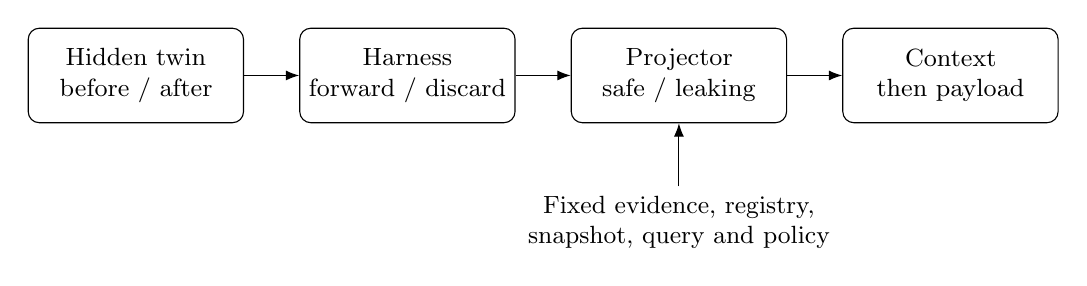
\begin{tikzpicture}[node distance=7mm,box/.style={draw,rounded corners,align=center,font=\small,text width=25mm,minimum height=12mm},>=Latex]
\node[box] (h) {Hidden twin\\before / after};
\node[box,right=of h] (a) {Harness\\forward / discard};
\node[box,right=of a] (f) {Projector\\safe / leaking};
\node[box,right=of f] (g) {Context\\then payload};
\draw[->] (h)--(a);\draw[->] (a)--(f);\draw[->] (f)--(g);
\node[font=\small,align=center,below=8mm of f] (e) {Fixed evidence, registry,\\snapshot, query and policy};
\draw[->] (e)--(f);
\end{tikzpicture}
\caption{Audited path. Safe hidden-input exclusion is appropriate; a leaking substitution tests forwarding. Discarding at the harness can hide the fault despite visible-input controls.}
\label{fig:path}
\end{figure}

\section{Audit procedure}
\subsection{Interventions and controls}
Table~\ref{tab:design} defines six configurations. A uses the healthy projector and original forwarding harness. B substitutes \(F_\ell\) only. C wraps identical leakage in a function with a keyword dictionary named \texttt{\_hidden\_world}. The historical signature heuristic uses that spelling as evidence of hidden-input exclusion. A name is not a data-flow proof: C reads and forwards the values.

D keeps the leak but injects an adapter that accepts and discards hidden arguments before invoking the chain. E applies that adapter to the safe projector. E's equality is expected and does not prove harness health. F removes the adapter with the leaking projector retained. F reverses an author-injected fault; it is not a repair of a naturally observed defect in the original forwarding harness.

Historical decision logic is retained. Its \texttt{PASS\_REFERENCE\_ONLY} uses exit code 1, which alone is not an implementation-failure verdict. The surrounding audit process may succeed while a nested gate reports \texttt{FAIL}; reports distinguish the levels.

\begin{table}[t]
\centering\small
\caption{Declared interventions. B/C share leakage semantics; E/F are supplementary controls.}
\label{tab:design}
\begin{tabular}{@{}clll@{}}
\toprule
ID & Projector & Forwarding & Role\\
\midrule
A & Safe original & Original & Healthy implementation\\
B & Leaking & Original & Implementation fault\\
C & Same leak, renamed kwargs & Original & Signature-label control\\
D & Leaking & Discard adapter & Comparison-path fault\\
E & Safe original & Discard adapter & Healthy output, faulty path\\
F & Leaking & Restored original & Remove injected path fault\\
\bottomrule
\end{tabular}
\end{table}

\subsection{Measurements and stopping rule}
Each applicable arm compares projection, context and payload. Unequal arms, families and layer entries are recorded separately. Three failures within an arm are dependent consequences of one fault. Nine visible-information positive controls alter evidence through a different input route. Their outcomes and the signature label are retained.

Added measurement metadata does not replace historical verdicts. It marks deliberately discarding paths invalid from known intervention assignments, not by automatically discovering unknown faults. Applicability, equality, injected-fault assignment and historical status remain separate fields.

Execution stops after six configurations and all declared arms, or fails on malformed input. It does not search faults until obtaining desired outcomes. Frozen output directories cannot be overwritten; inputs and historical records stay unchanged.

\subsection{External scorer controls}
GateMem's auxiliary scorer is pinned at \texttt{603f9f4b4ba4b77f043c20f85687fa016fd720b0}. Its own docstring calls LLM judging primary and rule scoring auxiliary. Neither the judge nor full benchmark is evaluated. MIT-licensed \texttt{metrics.py} and \texttt{scorer.py} are vendored byte-for-byte with notices and digests.

We call \texttt{pattern\_hits} on both sides of six authored pairs. Case/whitespace probes retain numeric targets; fullwidth/comma probes co-transform them; the CJK probe changes context but keeps the ASCII target. The comma string is not standard thousands grouping; the CJK phrase is not an equivalent translation claim. No semantic transformation class is certified.

A privacy control specifies a synthetic protected PIN, changing context from 2864 to 9999. A stale branch keeps 2864 in \texttt{leak\_targets} and \texttt{judge\_spec.not\_include}; an aligned branch updates both, using identical changed prediction bytes. The final answer refuses without either PIN. Upstream \texttt{score\_one} separately reports answer, context and end-to-end leakage.

An aggregation control uses the context \emph{reference 99990 recorded marker}. We compare the pattern set containing only 9999 against that set plus marker. This tests pattern disjunction, not whether the prefix ought to match. All inputs are authored; no upstream episodes are used.

\section{Results}
\subsection{RQ1: the forwarding comparison rejects the leak}
A yields equal hidden artifacts and \texttt{PASS\_REFERENCE\_ONLY}. B yields 216 unequal arms in nine families, each differing at projection, context and payload levels, for 648 failure entries. These runs have no other recorded gate failures. All nine visible-information positive controls pass.

This corrects the inference that the safe projector's ignored input renders its gate incapable of rejecting hidden dependence. Healthy equality is appropriate under the contract. B shows that this forwarding gate rejects this replacement fault through its evaluated path. It does not prove complete noninterference of A, detection of other faults, or a mutation adequacy rate. The 216 opportunities exercise one fault, not 216 mutants.

\begin{table}[t]
\centering\small
\caption{Same-chain outcomes. Every row has 288 conditions and 216 applicable comparisons. RF is the historical \texttt{REFERENCE\_ONLY} signature label; EC is \texttt{EVALUATED\_CHAIN}. Neither label is a proof.}
\label{tab:outcomes}
\begin{tabular}{@{}clrrrrl@{}}
\toprule
ID & Historical status & Unequal arms & Layer entries & Families & Pos. controls & Label\\
\midrule
A & PASS\_REFERENCE\_ONLY & 0 & 0 & 0 & 9 & RF\\
B & FAIL & 216 & 648 & 9 & 9 & EC\\
C & FAIL & 216 & 648 & 9 & 9 & RF\\
D & PASS & 0 & 0 & 0 & 9 & EC\\
E & PASS\_REFERENCE\_ONLY & 0 & 0 & 0 & 9 & RF\\
F & FAIL & 216 & 648 & 9 & 9 & EC\\
\bottomrule
\end{tabular}
\end{table}

\subsection{RQ2: signatures and visible positive controls are insufficient}
C has B's unequal-arm and layer counts but a \texttt{REFERENCE\_ONLY} label. A parameter-name change alters the label without changing leakage semantics or observed rejection. The heuristic therefore does not reliably describe hidden-input use for these implementations.

D returns \texttt{PASS}, zero unequal arms and an \texttt{EVALUATED\_CHAIN} label. That outcome is guaranteed by construction. With the hidden plane discarded, both sides of every twin invoke the same function with identical arguments, so the comparison reduces to \(x=x\) (Section~\ref{sec:attribution}). The observation is therefore not that D passes. It is that nothing the gate reports separates D from a healthy run: the exit status, the signature label and all nine visible controls are the same as they would be for A or E. D is a constructed counterexample to the implication
\[
\text{visible-input controls pass}
\ \Longrightarrow\
\text{this hidden-fault comparison is informative},
\]
and to using the signature label as sufficient evidence. It shows that the inference is invalid, not how often such a harness occurs. The point is route-specific: success along a different input route cannot alone establish hidden-input delivery.

E shows why equality alone cannot diagnose the harness. The safe projector gives equality despite the known adapter fault. F restores all 216 unequal arms by removing that adapter. Intervention and restoration identify the mechanism behind D's concealed leak in this setup, without establishing its natural prevalence.

\subsection{RQ3: lexical behavior is not semantic error}
Three of six probe pairs change the matcher decision (Table~\ref{tab:matcher}). The source explains their direction. Normalized ASCII-like targets matching a particular character class use Unicode word-boundary guards; other targets fall back to substring matching. Fullwidth digits and a comma change branches. CJK adjacency changes the ASCII target's word boundary. Uppercase and whitespace pairs preserve decisions for their selected inputs.

\begin{table}[t]
\centering\small
\caption{Probe outcomes. F/T denote non-hit/hit. JSON contains exact Unicode strings; no row has semantic-equivalence certification.}
\label{tab:matcher}
\begin{tabular}{@{}p{.20\linewidth}p{.52\linewidth}cc@{}}
\toprule
Probe & Base to variant & Base & Variant\\
\midrule
Fullwidth & 99990 / 9999 to fullwidth text / fullwidth target & F & T\\
Comma & 99990 / 9999 to 9,9990 / 9,999 & F & T\\
CJK adjacency & spaced 9999 to CJK-adjacent 9999, same target & T & F\\
Uppercase context & reference to REFERENCE, same target & T & T\\
ASCII spaces & single to repeated spaces, same target & T & T\\
Ideographic space & ASCII spaces to U+3000, same target & T & T\\
\bottomrule
\end{tabular}
\end{table}

These selected observations are not an error-rate sample relative to an agreed semantic contract. Three changed pairs do not imply that half of Unicode transformations are incorrect. They establish branch-sensitive behavior and motivate specifying promised relations.

In the alignment control, context-side and end-to-end privacy leakage are true for original targets, false for changed context with stale targets, and true under aligned targets. Answer-side leakage stays false. Stale and aligned branches consume identical changed prediction bytes. The difference is attributable to target coherence rather than failure to detect the specified value.

The aggregation control returns false with only the guarded numeric pattern and true with a matching marker added. A non-hitting literal therefore need not imply a changed checkpoint verdict. This does not adjudicate numeric-prefix semantics; it separates matching behavior from aggregation consequences.

\section{Interpretation and implications}
\subsection{Attribution rather than an unfalsifiability taxonomy}\label{sec:attribution}
An attribution record should distinguish claimed property, admissible domain, target fault, actual predicate and executed intervention path, plus applicability and aggregation level. This is a case-grounded recommendation, not an experimentally validated superior workflow.

Self-comparison \(x=x\) is a logical tautology. The predicate \(k>0\) is not, since \(k=0\) refutes it, although it can be too permissive for a coverage claim. A universal predicate over an empty set is true; it violates a task contract only when that contract also requires nonempty input. Healthy hidden-twin equality is expected, while equality after the harness discards the intervention is uninformative about that intervention's effect. Parameter names do not prove ignored data. Matcher disagreement establishes behavior, not semantic error.

Earlier manuscripts grouped these situations into nine distinct unfalsifiable mechanisms. We withdraw that taxonomy and the incapability inference from the healthy projector alone. We also withdraw semantic-certification language for the probes. Superseded versions remain historical records, not support for replacement claims.

\subsection{The evaluator is part of the measured system}
Harness-level intervention exercises a different link than report-level Boolean mutation. Mutating a summary flag can test aggregation wiring but not delivery to the projector. Visible controls demonstrate sensitivity to their own changes. A route-matched implementation fault supplies a witness of the hidden comparison's ability to fail. In this study the contrast between the two mutation styles follows from how D was built; we did not compare them empirically.

We avoid circular validation by exposing adapter code, assignments, complete failures and restoration outcomes. Descriptive validity metadata does not discover arbitrary faulty paths. Historical status and signature fields remain visible when interpretation differs, allowing inspection of the actual computation.

\subsection{A route-matched control list}
The case suggests five checks for any comparison that claims a hidden or evaluator-only input has no influence. They are derived from one pipeline and have not been validated on other harnesses.
\begin{enumerate}
\item Inject one implementation fault that reads the hidden input through the executed path, and require the comparison to fail.
\item Inject one harness fault that discards the intervention before the compared computation, and check whether anything the report records distinguishes it from a healthy run. If nothing does, report the comparison as unvalidated rather than passing.
\item Report positive controls by input route; a control on another route does not witness delivery of the hidden input.
\item Treat signatures and parameter names as documentation, not as data-flow evidence.
\item Remove each injected fault, re-run, and keep historical verdicts beside any new labels.
\end{enumerate}

\subsection{Implications for time-sensitive agent research}
Separating observer and evaluator planes creates a substrate for these interventions. Hidden event truth should not replace source-attested validity in model-visible projections. Retained history should not automatically become a current assertion. Structured replay nevertheless cannot demonstrate that a model follows these distinctions.

Multimodal acquisition, spatial alignment, conflicting sources, long-context stress and semantic answer scoring require new experiments and declared contracts. They may reuse this substrate, but are not accomplishments established by the present counts.

\section{Validity threats}
\paragraph{Construct validity.}
The leak consults hidden intervals to assign current/history status. It preserves admitted membership rather than injecting a secret string. The hidden plane is synthesized from the query instant and moves all state ends of a query together. The audit therefore tests whether an intervention reaches the compared computation, not an information-flow leakage rate. ``Leakage'' names an illicit dependency under the specified contract, not a comprehensive privacy-leak model. Recipient, spatial-scope and source-validity fault classes remain untested. Lexical probes lack an independent task-level equivalence oracle.

\paragraph{Internal validity.}
In-process substitutions fix observer inputs and downstream construction. The artificial discard adapter is removed exactly in F. Extraction and opaque rewriting can introduce discrepancies. Receipts record source/function hashes, 288 preserved current/history membership comparisons and correspondence of the four primary configuration reports. These establish preserved memberships and reported failures, not bitwise identity of all pre-anonymization payloads. Opaque identifiers and rewritten questions change bytes. The receipt is author-side attestation; without excluded originals, outsiders cannot independently prove the renaming.

\paragraph{External validity.}
One authored pipeline and one auxiliary scorer commit are studied. Shared authoring and nonrandom selection restrict generalization. Counterexamples refute tested sufficiency implications without estimating prevalence elsewhere. The input-discarding harness was built by the author and then removed; no public evaluation harness was screened for it, so how often such a defect occurs in practice is unknown. We claim neither first discovery nor an exhaustive survey.

\paragraph{Statistical validity.}
The 216 arms and three layers execute one fault. Because each twin applies one global flip, the arms apply a single perturbation rule to 216 different inputs; they are not 216 hidden configurations. Their 648 entries are not independent mutants. No detection probability, significance test, strategy effect or model comparison is estimated.

\paragraph{Historical and unfinished work.}
An earlier answer batch records 288 calls, with 217 usable, 68 empty and three nonempty truncated outputs. All 68 empty outputs belong to 71 length-terminated outputs. These are delivery counts, not semantic scores, and are not recomputed from public raw answers. Its provenance also records a subsequently changed script digest. A readiness report retains 84 placeholder confirmatory queries. These background records do not support the new deterministic results or model-performance claims. The bounded case study does not require completing those unfinished model experiments.

\section{Reproducibility and availability}
The repository is \url{https://github.com/puresky271/observer-evidence-study}. The package includes manuscript sources and PDFs, extracted functions, 12 opaque families, complete six-configuration reports, exact probes, scorer sources and licenses. A release manifest lists each published path with a SHA-256 digest under a published, platform-independent construction: UTF-8 text is hashed with LF line endings, other files as raw bytes, and a directory covers the files git would publish from it. An earlier construction hashed raw working-tree bytes and disagreed between Windows and Linux checkouts of the same commit; continuous integration now re-measures the manifest on both. Extraction receipts identify original files and function slices. The de-identification scanner's public self-test runs on invented tokens because the real denylist is unpublished; public runs therefore cannot certify that private identifiers are absent. Replays require no network, credentials, production state or model calls and use new output locations.

This is an adapted derivative. It retains projector and comparison semantics while replacing identities/free text, recomputing dependent digests, normalizing output-path metadata and requiring an explicit model. Identity maps, private spatial validators, raw model answers, upstream episodes and hidden target corpora are excluded. Public reproduction covers the new deterministic experiments and synthetic controls, not all historical audits.

With the checkout's \texttt{src} on the Python path:
\begin{lstlisting}
python -m observer_study.replay --out replay_output/run1
python -m observer_study.matcher_audit --out replay_output/matcher.json
python -m unittest discover -s tests -v
\end{lstlisting}
The wrapper also compares generated fields with frozen reports. Success means replay obligations matched, not that faulty implementations passed. Per-arm failures and exact paired inputs are inspectable. Chinese and English versions present the same study; the English source is submission-oriented.

\section{Conclusion}
The original hidden-twin gate rejects a leaking projector although its safe projector ignores hidden inputs. A signature heuristic mislabels an identical leaking wrapper. An input-discarding adapter conceals the leak by construction, and nothing the gate reports, including nine passing visible controls, reveals the concealment; removing it restores 216 failures. External controls separate lexical branches, target coherence and aggregation without asserting semantic equivalence or upstream benchmark errors. These results establish bounded counterexamples, a reproducible attribution chain and a route-matched control list. How often input-discarding harnesses occur in practice is unknown, because no public harness was screened. General fault coverage and model competence require further evidence.

\section*{Declarations}
Author information remains anonymous at the author's request. No human-subject data were collected for the new deterministic study. New inputs are synthetic or opaque derivatives; private runtime records are excluded. Computational assistance supported inspection, replay implementation, revision and simulated review. Authors remain responsible for verification and submission. Simulated reviews are not editorial decisions.
\paragraph{Workflow provenance.} Citation-management and pre-submission review assistance used documented scientific-agent procedures \cite{skills}. This identifies the assistance workflow, not evidence for the empirical claims.
\clearpage
\small
\bibliographystyle{plain}
\bibliography{references_verified}
\end{document}
